\documentclass[10 pt]{beamer}
\usepackage[spanish]{babel}
\usepackage{amsmath}
\usepackage{amsfonts}
\usepackage{amssymb}
\usepackage{graphicx}
\usepackage{parskip}
\usetheme{Madrid}

\title[Ecuaciones Diferenciales]{\large{Ecuaciones Diferenciales y Problemas con Valores en la Frontera}}
\subtitle[Libro]{\large{Libro de Nagle, Saff y Snider}}
\author{Grupo 2}
\institute[UNMSM]{
    \Large{Universidad Nacional Mayor de San Marcos} \\
    \vspace{2mm}
    \large{Facultad de Ingeniería de Sistemas e Informática}
    \vspace{2.3cm}
}
\date{Mayo 2024}

\begin{document}

\begin{frame}
    \titlepage
    \vspace*{-3.9cm}
    \begin{center}
        
\includegraphics[scale=0.1]{./logo/logo.png}
    \end{center}
\end{frame}

\section{3.3 Calentamiento y Enfriamiento de Edificios}
\begin{frame}{3.3 Calentamiento y Enfriamiento de Edificios}
    \begin{enumerate}[\footnotesize{8}]
        \item Una cochera sin calefacción ni aire acondicionado tiene una constante de tiempo de 2 horas. Si la temperatura exterior varía como una onda senoidal con un mínimo de $50^\circ \text{F}$ a las 2:00 A.M. y un máximo de $80^\circ \text{F}$ a las 2:00 P.M., determine los instantes en que el edificio alcanza sus temperaturas máxima y mínima, suponiendo que el término exponencial se extingue
    \end{enumerate}

    \begin{block}{Solution}
        La función de onda senoidal :
        \begin{equation}
            M(t) = M_o - B\cos(\omega t)
        \end{equation}

        Ley de enfriamiento de Newton :
        \begin{equation}
            \dfrac{dT}{dt} = k \bigg( M(t) - T(t) \bigg) + H(t) + U(t)
        \end{equation}

        Se tiene la temperatura máxima y mínima:
        \begin{equation}
            M_o = \dfrac{T_{\text{max}} + T_{\text{min}}}{2}
        \end{equation}
    \end{block}
\end{frame}

\begin{frame}
    \begin{block}{Solution}
        Reemplazando los datos en (3)
        \begin{equation*}
            M_o = \dfrac{80 + 50}{2}
        \end{equation*}
        \begin{equation}
            M_o = \dfrac{80 + 50}{2} = 65^\circ \text{F}
        \end{equation}

        Reemplazando (4) en (1)
        \begin{equation*}
            M(t) = M_o - B\cos(\omega t)
        \end{equation*}
        \begin{equation*}
            M(t) = 65 - B\cos(\omega t)
        \end{equation*}

        Para un t(0)
        \begin{align*}
            50 & = 65 - B\cos(\omega 0) \\
            B  & = 15
        \end{align*}
        \begin{equation}
            M(t) = 65 - 15\cos(\omega t)
        \end{equation}
    \end{block}
\end{frame}

\begin{frame}
    \begin{block}{Solution}
        La frencuencia angular es:
        \begin{equation}
            \omega = \dfrac{2\pi}{T} = \dfrac{2\pi}{24} = \dfrac{\pi}{12}
        \end{equation}

        Reemplazando (6) en (5)
        \begin{equation}
            M(t) = 65 - 15\cos\bigg(\dfrac{\pi}{12}t\bigg)
        \end{equation}

        Luego H(t) = U(t) = 0, reemplazando (7) en (2),
        \begin{equation*}
            \dfrac{dT}{dt} = k \bigg( M(t) - T(t) \bigg) + H(t) + U(t)
        \end{equation*}
        \begin{equation*}
            \dfrac{dT}{dt} = k \bigg(65 - 15\cos\bigg(\dfrac{\pi}{12}t\bigg) - T(t) \bigg)
        \end{equation*}
        \begin{equation}
            \dfrac{dT}{dt} + kT(t) = k \bigg(65 - 15\cos\bigg(\dfrac{\pi}{12}t \bigg) \bigg)
        \end{equation}
    \end{block}
\end{frame}

\begin{frame}
    \begin{block}{Solution}
        Luego, el factor integrante es
        \begin{equation*}
            \mu(t) = e^{\int kdt}
        \end{equation*}
        \begin{equation}
            \mu(t) = e^{kt}
        \end{equation}

        Multiplicamos el factor integrante (9) en (8)
        \begin{equation}
            e^{kt}\dfrac{dT}{dt} + e^{kt}kT(t) = e^{kt}k \bigg(65 - 15\cos\bigg(\dfrac{\pi}{12}t \bigg) \bigg)
        \end{equation}

        Agrupamos los terminos
        \begin{equation}
            \dfrac{d}{dt} \bigg[e^{kt}T(t)\bigg]  = e^{kt}k \bigg(65 - 15\cos\bigg(\dfrac{\pi}{12}t \bigg) \bigg)
        \end{equation}

        Integramos
        \begin{equation}
            e^{kt}T(t)= k \int e^{kt} \bigg(65 - 15\cos\bigg(\dfrac{\pi}{12}t \bigg) \bigg)dt + C
        \end{equation}
    \end{block}
\end{frame}

\begin{frame}
    \begin{block}{Solution}
        Se tiene
        \begin{equation}
            T(t)= e^{-kt} \int e^{kt} k\bigg[65 - 15\cos\bigg(\dfrac{\pi}{12}t \bigg) \bigg]dt + Ce^{-kt}
        \end{equation}

        La ecucación seria
        \begin{equation}
            T(t)= 65 - 15e^{-kt} \int e^{kt} k\bigg[\cos\bigg(\dfrac{\pi}{12}t \bigg) \bigg]dt + Ce^{-kt}
        \end{equation}

        Luego resolvemos la integral
        \begin{equation}
            e^{kt}cos\bigg(\dfrac{\pi}{12}t\bigg) + \dfrac{\pi}{12k}e^{kt}\sin\bigg(\dfrac{\pi}{12}t\bigg) - \dfrac{\pi^{2}}{144k^{2}}\int e^{kt} k\bigg[\cos\bigg(\dfrac{\pi}{12}t \bigg) \bigg]dt
        \end{equation}
        \begin{equation}
            = \int e^{kt} k\bigg[\cos\bigg(\dfrac{\pi}{12}t \bigg) \bigg]dt
        \end{equation}

        La integral seria
        \begin{equation}
            \dfrac{144k^{2}}{144k^{2} + \pi^{2}} \bigg[e^{kt}cos\bigg(\dfrac{\pi}{12}t\bigg) + \dfrac{\pi}{12k}e^{kt}\sin\bigg(\dfrac{\pi}{12}t\bigg) \bigg]
        \end{equation}
    \end{block}

\end{frame}

\begin{frame}
    \begin{block}{Solution}
        La ecuación general seria:
        \begin{equation}
            T(t) = 65 - \dfrac{2160k^{2}}{144k^{2} + \pi^{2}} \cos\bigg(\dfrac{\pi}{12}t\bigg) - \dfrac{180\pi k}{144k^{2} + \pi^{2}} \sin\bigg(\dfrac{\pi}{12}t\bigg) + Ce^{-kt}
        \end{equation}

        Reemplazamos $k = \dfrac{1}{2}$
        \begin{equation}
            T(t) = 65 - \dfrac{540}{36 + \pi^{2}} \cos\bigg(\dfrac{\pi}{12}t\bigg) - \dfrac{90\pi}{36 + \pi^{2}} \sin\bigg(\dfrac{\pi}{12}t\bigg) +  Ce^{-\frac{t}{2}}
        \end{equation}

        El término exponencial se extingue.
        \begin{equation}
            T(t) = 65 - \dfrac{540}{36 + \pi^{2}} \cos\bigg(\dfrac{\pi}{12}t\bigg) - \dfrac{90\pi}{36 + \pi^{2}} \sin\bigg(\dfrac{\pi}{12}t\bigg)
        \end{equation}
    \end{block}
\end{frame}

\begin{frame}
    \begin{block}{Solution}
        Para hallar el mínimo y el máximo derivamos
        \begin{equation}
            \dfrac{dT}{dt} = \pi\cos\bigg(\dfrac{\pi}{12}t\bigg) - 6\sin\bigg(\dfrac{\pi}{12}t\bigg) = 0
        \end{equation}

        Se tiene
        \begin{equation}
            t = \dfrac{12}{\pi} \arctan\bigg(\dfrac{\pi}{6}\bigg) = 1.84
        \end{equation}

        El tiempo de la temperatura máxima y mínimo son
        \begin{align*}
            T_\text{min} & = 1.84 \text{ horas}                      \\
            T_\text{max} & = t_\text{min} + 12 = 13.84 \text{ horas}
        \end{align*}

        Reemplazamos en (20), por lo tanto la temperatura mínima de $T(min) \approx 51.7^{\circ} F$, se alcanzará 1.84 horas después de las 2:00 A.M. es decir a las 3:50 A.M. \\

        Y para la temperatura máxima de $T(max) \approx 78.3^{\circ} F$, se alcanzará 12 horas después es decir a las 3:50 P.M.
    \end{block}
\end{frame}

\begin{frame}
    \begin{block}{Solution}
        Graficando la ecuación T(t)
        \begin{figure}[H]
            \vspace*{0.2cm}
            \centering
            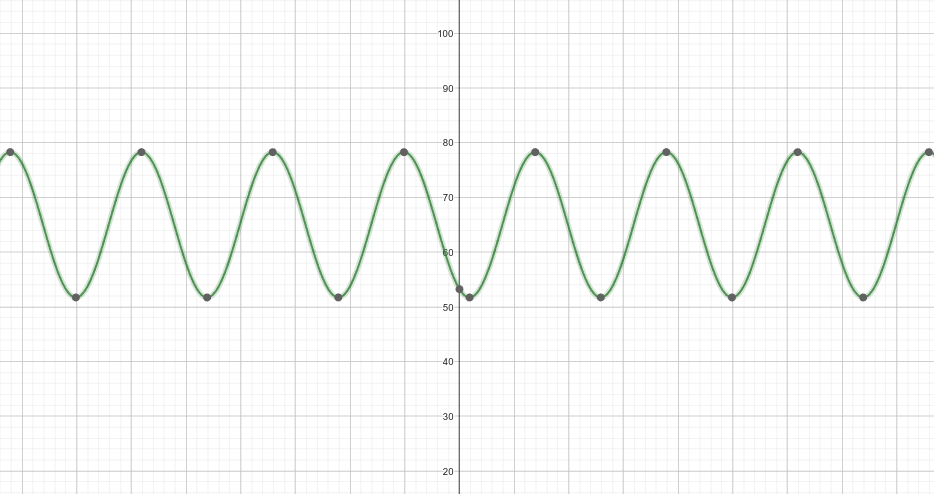
\includegraphics[scale=0.5]{"./img/Grafica.png"}
            \caption{Grafica T(t)}
            \label{Grafica 1}
        \end{figure}
    \end{block}
\end{frame}

\setcounter{equation}{0}

\section{3.3 Calentamiento y Enfriamiento de Edificios}
\begin{frame}{3.3 Calentamiento y Enfriamiento de Edificios}
    \begin{enumerate}[{12}]
        \item Dos amigos se sientan a platicar y disfrutar una taza de café. Al servir el café, el amigo impaciente agrega de inmediato una cuchara de crema a su café. El amigo relajado espera 5 minutos antes de añadir una cuchara de crema (que se ha mantenido a temperatura constante). Es entonces cuando ambos comienzan a tomar el café. ¿Quién tiene el café más caliente? Suponga que la crema está más fría que el aire y use la ley de enfriamiento de Newton.
    \end{enumerate}

    \begin{block}{Solution}
        Ley de enfriamiento de Newton
        \begin{equation}
            \dfrac{dT}{dt} = k \bigg( M(t) - T(t) \bigg) + H(t) + U(t)
        \end{equation}

        Supongamos que $T_1(t)$ y $T_2(t)$ son la temperatura del café del amigo impaciente y relajado respectivamente, donde t = 0 significa la hora en que sirvió el café. La temperatura del aire $M(t) = M_o$
        \begin{equation}
            T_k(t) = M_o + C_ke^{-kt},\quad k = 1,2
        \end{equation}
    \end{block}
\end{frame}

\begin{frame}
    \begin{block}{Solution}
        Las constante C, dependen de las temperatura iniciales del café. Supongamos que la temperatura del café cuando se sirvió fue $T_o$, la cantidad de café pedida fue $V_o$, la temperatura de la crema era $T_c$ y la cuchara tenía capacidad de $V_c$. Luego, tenemos las condicionales iniciales.
        \begin{equation*}
            T_2(0) = T_o \quad,\quad T_1(0) = \dfrac{T_o V_o + T_c V_c}{V_o + V_c}
        \end{equation*}

        Reemplazamos en (2)
        \begin{equation*}
            C_2 = T_o - M_o \quad,\quad C_1 = \dfrac{T_oV_o + T_cV_c}{V_o + V_c} - M_o
        \end{equation*}

        Se tiene
        \begin{align*}
            T_1(t) & = M_o + \bigg (\dfrac{T_oV_o + T_cV_c}{V_o + V_c} - M_o \bigg) e^{-kt} \\
            T_2(t) & = M_o + (T_o - M_o)e^{-kt}
        \end{align*}
    \end{block}

\end{frame}

\begin{frame}
    \begin{block}{Solution}
        Después de 5 min
        \begin{align*}
            T_1(5) & = M_o + \dfrac{(T_oV_o + T_cV_c) - M_o(V_o + V_c)}{V_o + V_c} e^{-k5} \\
            T_2(5) & = M_o + (T_o - M_o)e^{-5k}
        \end{align*}

        En ese mismo instante, el amigo relajado había añadido una cucharadita crema reduciendo la temperatura de su café a
        \begin{equation}
            \widetilde{T}_2(5) = \dfrac{T_2(5)V_o + T_cV_c}{V_o + V_c} = \dfrac{[M_o + (T_o - M_o)e^{-5k}]V_o + T_cV_c}{V_o + V_c}
        \end{equation}

        Ahora comparamos $T_1(5)$ y $\widetilde{T}_2(5)$
        \begin{equation}
            T_1(5) - \widetilde{T}_2(5) = (V_o + V_c)^{-1} V_c(M_o - T_c) (1 - e^{-5k}) > 0
        \end{equation}

        Como la crema es más fría que el aire, es decir $T_c < M_o$. Así, el amigo impaciente tomó el café más caliente.
    \end{block}
\end{frame}

\setcounter{equation}{0}

\section{3.5 Circuitos Eléctricos}
\begin{frame}{3.5 Circuitos Eléctricos}
    \begin{enumerate}[{6}]
        \item Deduzca una ecuación de equilibrio de la potencia para los circuitos RL y RC. (Ver problema 5). Analice el significado de los signos de los tres términos de potencia.
    \end{enumerate}
    \begin{block}{Solution}
        Para un circuito RL tenemos
        \begin{equation}
            L \dfrac{dI}{dt} + RI = E(t)
        \end{equation}

        Multiplicamos (1) por I para
        \begin{align*}
            L \dfrac{dI}{dt}I + RI^2 = EI \\
            \dfrac{d}{dt} \bigg( \dfrac{1}{2} LI^2 \bigg) + RI^2 = EI
        \end{align*}

        La potencia generada por la fuente es igual a la potencia insertada en el inductor más la potencia disipada por la resistencia.
    \end{block}
\end{frame}

\begin{frame}
    \begin{block}{Solution}
        Para un circuito RC tenemos
        \begin{equation}
            R \dfrac{dq}{dt} + \dfrac{q}{C} = E
        \end{equation}

        Multiplicamos (2) por I para
        \begin{equation}
            RI \dfrac{dq}{dt} + I \dfrac{q}{C}= EI
        \end{equation}

        Reemplazamos I por $\dfrac{dq}{dt}$ y q por $CE_c$ en (3)
        \begin{align*}
            RI^2 + \dfrac{dq}{dt} CE_c = EI \\
            RI^2 + \dfrac{d}{dt} \bigg (\dfrac{1}{2} CE_c^2 \bigg) = EI
        \end{align*}

        La potencia generada por la fuente de voltaje es igual a la potencia insertada en el capacitor más la potencia disipada por la resistencia.
    \end{block}
\end{frame}

\end{document}
